
%%% Application Domain Analysis %%%
\chapter{Application domain analysis}
This chapter contains a application domain analysis. The purpose of the analysis is to understand how Labelless Media is going to use the system and thereby specify the user requirements for the system. This includes: 
\begin{itemize}
  \item Identifying actors
  \item Defining use cases
  \item Identifying the functions of the system
  \item Determining the user requirements
\end{itemize}

\section{Actors}
To get a better understanding of the users and an overview of their possible usage of the system, the actors are investigated. The system has two actors which are user and superuser. These actors are respectively a salesperson and a company owner. The only difference between the two actors is that only a company owner or the superuser can remove and create users. To illustrate the actors opportunities on the webpage, statechart diagrams for the user and the superuser are made.
\newline \newline \noindent
For both actors the user experience starts with opening the webpage and logging in. If the login gets rejected, it returns to the login page. \newline \newline \noindent
\textbf{User} can administrate the filter, clients and leads. After a user finishes their current tasks, they can either close the webpage and end the session, or log off and return to the login page. The user may close the webpage at any time during the session. The statechart diagram for the user is seen in Figure \ref{fig:statechartMember}.
\newline
\begin{figure}[H]
    \centering
    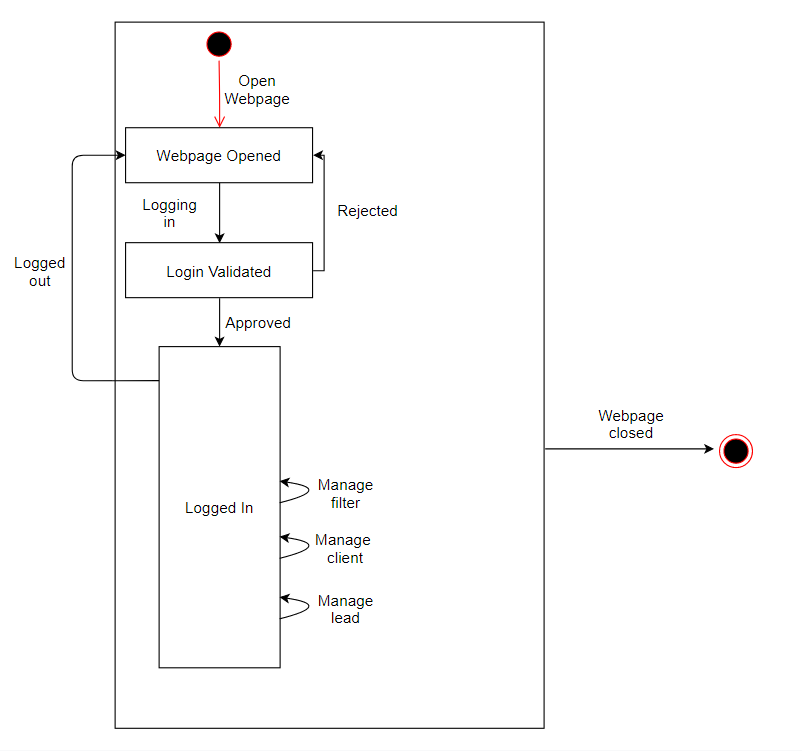
\includegraphics[scale=.7, clip]{figures/useCaseMember.png}
    \caption{Statechart diagram for a user}
    \label{fig:statechartMember}
\end{figure}
\noindent
\textbf{Superuser} is also able to manage the filter, clients and leads. The difference between user and superuser is that the superuser can also manage users. This role is created in order to add and remove users if necessary. The statechart diagram for the superuser is seen in Figure \ref{fig:statechartAdmin}.
\begin{figure}[H]
    \centering
    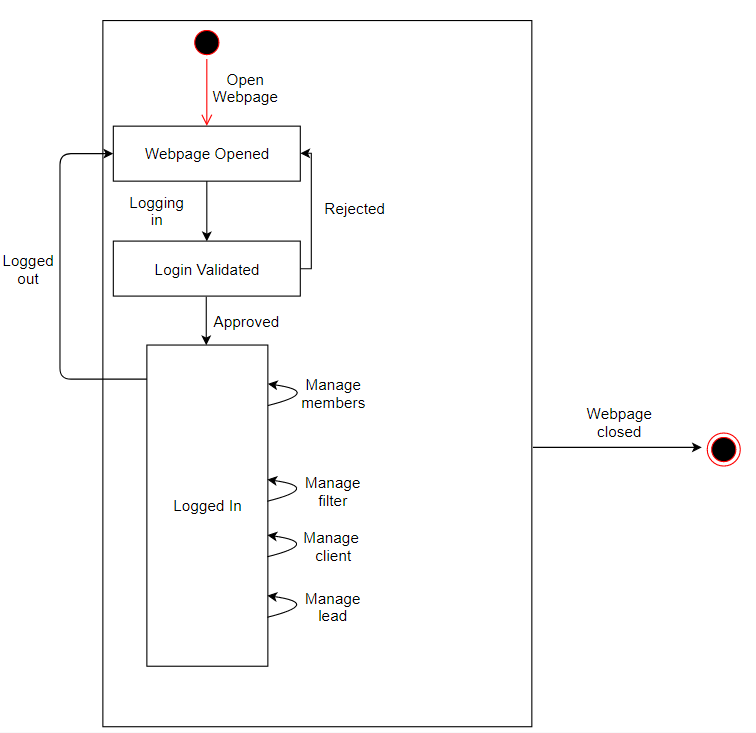
\includegraphics[scale=.7, clip]{figures/useCaseAdmin.png}
    \caption{Statechart diagram for an superuser}
    \label{fig:statechartAdmin}
\end{figure}

\section{Usage}
To get a better understanding of how the actors use the system, a table of use cases and actors is created.
The table illustrates the use cases and which actors are involved in the different use cases. The use case table can be seen in Table \ref{tab:useCaseTable}
\newline \newline \noindent
\textbf{Use cases}\newline
\begin{table}[]
\begin{tabular}{|l|l|l|}
\hline
\textbf{Use cases}         & superuser & user \\ \hline
Login                      & X     & X      \\ \hline
Accept lead                & X     & X      \\ \hline
Deny lead                  & X     & X      \\ \hline
Change lead icon           & X     & X      \\ \hline
Change leads description   & X     & X      \\ \hline
Finish lead                & X     & X      \\ \hline
Change password            & X     & X      \\ \hline
Manage filter criteria     & X     & X      \\ \hline
Add user                   & X     &        \\ \hline
Remove user                & X     &        \\ \hline
Add new contact person     & X     & X      \\ \hline
\end{tabular}
\caption{Table over use cases, and their relation to the actors.}
\label{tab:useCaseTable}
\end{table}
\newpage
\noindent
In the section below, some of the use cases are described in further details. \newline \newline \noindent
\textbf{Login}\newline
Every time the web application opens, the user is prompted with a login page. The reason for this is to prevent unwanted people accessing the web application. The web application contains data that only the staff at Labelless Media are supposed to see. The use case for login can be seen in Figure \ref{fig:useCaseLogin}.
\begin{figure}[H]
    \centering
    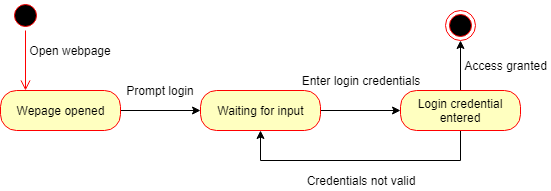
\includegraphics[scale=0.6, clip]{figures/useCaseLogin.png}
    \caption{Use case for login }
    \label{fig:useCaseLogin}
\end{figure}
\noindent
\textbf{Change lead icon}\newline
During the lifetime of a lead, it can change between different stages. These stages are illustrated by icons. All users are allowed to change the stage for the leads. A lead stage can be updated several times. The use case for a lead can be seen in Figure \ref{fig:useCaseChangeRequestIcon}.
\begin{figure}[H]
    \centering
    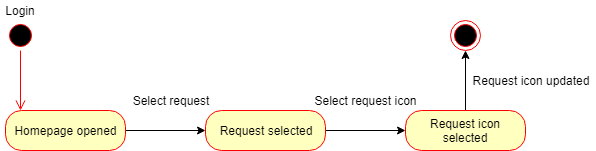
\includegraphics[scale=0.6, clip]{figures/useCaseChangeRequestIcon.png}
    \caption{Use case for changing the lead icon}
    \label{fig:useCaseChangeRequestIcon}
\end{figure}
\noindent
\textbf{Finish lead}\newline
When a lead is done, a user has to mark it as finished in the system which is shown in Figure \ref{fig:useCaseFinishRequest}. When a lead is marked as finished, the user is prompted with a review form where the user evaluates the job. When the lead is reviewed, the icon of the lead is updated, and the lead is marked as finished in the system.
\begin{figure}[H]
    \centering
    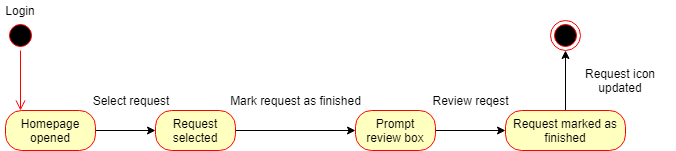
\includegraphics[scale=0.6, clip]{figures/useCaseFinishRequest.png}
    \caption{Use case for finishing a lead}
    \label{fig:useCaseFinishRequest}
\end{figure}
\noindent
\textbf{Change password for user}\newline
Whenever a user is logged in, the user is able to change its password. In order to change the password, the user has to type in the current password for validation.
\begin{figure}[H]
    \centering
    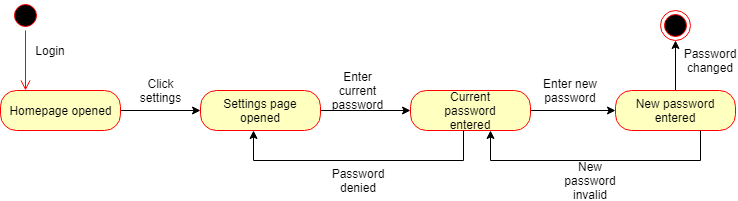
\includegraphics[scale=0.6, clip]{figures/useCaseMemberChangePassword.png}
    \caption{Use case for a user password change}
    \label{fig:useCaseMemberChangePassword}
\end{figure}
\noindent
\textbf{Change password as superuser}\newline
A superuser is able to change password for all users in the system. When a superuser changes a password for a user, the superuser must enter his own password as validation. 
\begin{figure}[H]
    \centering
    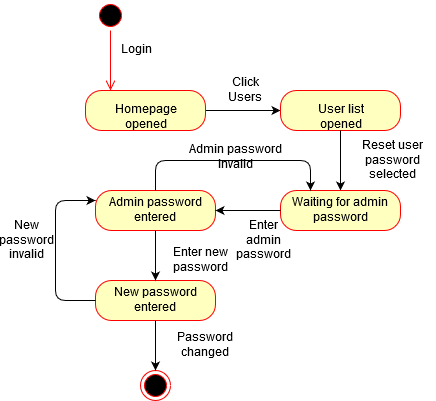
\includegraphics[scale=0.6, clip]{figures/useCaseChangePasswordAdmin.png}
    \caption{Use case for an superuser password change}
    \label{fig:useCaseAdminChangePassword}
\end{figure}
\noindent
\textbf{Add user}\newline
When a new user has to be added to the system, an superuser has to go through the process in Figure \ref{fig:useCaseAddMember}. First the superuser goes to his homepage, and selects the user list. Then the superuser inputs the relevant user data, and creates the new user.
\begin{figure}[H]
    \centering
    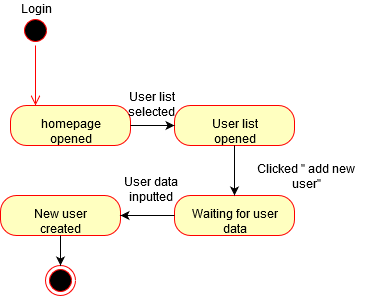
\includegraphics[scale=0.7, clip]{figures/useCaseAddMember.png}
    \caption{Use case for adding a new user}
    \label{fig:useCaseAddMember}
\end{figure}
\newpage

\section{Functions}
In this section the functions of the system will be identified and described. The focus of this section is what the system can do to assist the actors in their work. The functions are listed in Table \ref{tab:functionTable}, with their function type and complexity.
\begin{table}[H]
\begin{tabular}{|l|l|l|}
\hline
\textbf{Function name}  & \textbf{Complexity} & \textbf{Function type} \\ \hline
Login                             & Simple     & Update        \\ \hline
Log out                           & Simple     & Update        \\ \hline
Add user                          & Medium     & Update        \\ \hline
Remove user                       & Simple     & Update        \\ \hline
Change password                   & Simple     & Update        \\ \hline
Change lead icon                  & Simple     & Update        \\ \hline
Finish lead                       & Complex    & Update        \\ \hline
Deny lead                         & Simple     & Update        \\ \hline
Show leads                        & Complex     & Update        \\ \hline
Mark lead as contacted            & Simple     & Update        \\ \hline
Show lead information             & Medium     & Read          \\ \hline
Show client information           & Medium     & Read          \\ \hline
Add contact person to lead        & Simple     & Update        \\ \hline
Remove contact person from lead   & Simple     & Update        \\ \hline
Create meeting                    & Simple     & Update        \\ \hline
Cancel meeting                    & Simple     & Update        \\ \hline
Notify of meeting                 & Simple     & Signal        \\ \hline
Change display criteria           & Complex    & Read          \\ \hline
Add elements to blacklist         & Simple     & Update        \\ \hline
Remove elements from blacklist    & Simple     & Update        \\ \hline
\end{tabular}
\caption{Table over functions, their complexity and types.}
\label{tab:functionTable}
\end{table}
\noindent
The complex functions from the Table will be described below, to get a better understanding of how they work. 

\textbf{Show leads}

\textbf{Finish lead}

\textbf{Change display criteria}

%%% PACT Analysis %%%
\section{PACT analysis}
%%%%%%%%%%%%%%%%%%% INTRODUKTION  %%%%%%%%%%%%%%%%%%%%%%%%%%%%%%%%%%%%%
In this section a PACT analysis will be conducted in order to understand the users and their requirements for the system.
The purpose of the PACT analysis, is to get a overview of the people using the system, why they are using the system and the context which the system will be used in.

\subsection{People}
The intended users of the system are the sales personnel at Labelless Media. They are experienced in managing leads, communicating with clients, and used to using computerized systems, but with limited IT knowledge. The sales personnel all know Danish and English, but they have a strong preference towards the use of Danish. The sales personnel are the relation between Labelless Media and their potential clients. Besides this, the sales personnel also have other responsibilities. Therefore it is important that the system is simple, to minimize the time the sales personnel use to handle the leads. 
\newline \noindent

\subsection{Activities}
The overall purpose is to simplify the lead managing process and thus save time for the sales personnel. Currently, the sales personnel either receives emails with leads or cold calls a company to create one. The sales personnel then evaluates the leads and determines which leads look the most promising to Labelless Media and follow up on those first. According to the sales personnel this is a time consuming process and therefore they would like to have a system which helps them manage and process the leads. The system is supposed to give the lead a score, based on how promising it seems to Labelless Media. The system also  is supposed to give an overview over contacted and not contacted leads. Furthermore, the system is supposed to keep track of leads, both on-going and completed. When a lead is complete the salesman should be able to write how much Labelless Media earned on the lead.  The sales personnel is using a different system to organise their work, after a lead has turned into a job. This means that this system only covers the part of the process up until a contract is made and a lead is turned into a job.

\subsection{Context}
The sales personnel are working at the physical location of the company which allows them to discuss the leads with other employees of the company. It is possible, that the sales personnel update lead statuses or contact potential leads off site, when the salesman is having a meeting with a client. The sales personnel are tasked with analyzing potential leads, contacting companies about leads and keeping track of lead statuses, these activities are performed on company computers and phones. The salesman are managing leads across multiple software solutions.
The sales personnel use both computers to keep track of lead development and phones to contact potential leads.

\subsection{Technologies}
Currently the sales personnel only uses Macs, with external screens of varying sizes. Thus the system should be scalable to fit the different screen sizes. The system should be developed as a web application and to ensure that it will be accessible on all current OS, and devices that has access to the internet and a modern webbrowser. This is to forfill a wish from Labelless Media to be able to use tablets in the future, so the system should be able to facillitate this option. tablets


\section{Requirements}
This section contains the requirements for the system. The requirements are split into two categories; functional and non-functional requirements. The functional requirements are what system must be able to do. The non-functional requirements are the qualities the system must have. The different requirements will be categorised by using the MoSCoW rules. These rules categorises the requirements into four categories. 

\begin{itemize}
    \item Must have
    \item Should have
    \item Could have
    \item Want to have, but won't be implemented. 
\end{itemize}

\subsection{Functional requirements}

\begingroup
\renewcommand{\arraystretch}{1.5} % Default value: 1


\begin{tabu} to \textwidth {|l | m{2cm} | X |}
\hline
Iteration & MoSCoW & Requirement \\ \hline
  0       &   M    &  Automatically create leads                \\ \hline
  0       &   M    &  Manually create leads                    \\ \hline
  0       &   M     &  Edit information regarding the leads      \\ \hline 
  0       &   S    &  Categorize leads into different stages    \\ \hline
  0       &   W  &  Delete leads                              \\ \hline
  0       &   M  &  Automatically rank leads \\ \hline
  0       &   W  &  Decline leads\\ \hline
  0       &   W  &  Send a notification when there are x days until a meeting is taking place  \\ \hline
  0       &   C  &  Send a notification when a client should be contacted again after a consideration period  \\ \hline
  0       &   S  &  Send a notification with a daily update on what activities happened the day before               \\ \hline
  0       &   C  &  Export meetings to Google Calendar               \\ \hline
  0       &   S  &  The application should be able to show statistics about sales personnel's performance  \\  \hline
0         &   W  &  Affect the ranking of leads by blacklisting criterias \\ \hline
0         &   S  &  User management \\ \hline
  
\end{tabu}
\endgroup

\subsection{Non-functional requirements}
\begingroup
\setlength{\tabcolsep}{6pt} % Default value: 6pt
\renewcommand{\arraystretch}{1.5} % Default value: 1
\begin{tabu} to \textwidth {|l | m{2cm} | X |}
\hline
Iteration & MoSCoW & Requirement \\ \hline
0         &   M    & The user interface is designed for danish employees and the components should therefore be displayed in Danish with æ, ø, å  \\ \hline
0         &   M  & The web application should give an overview of the leads \\ \hline
0         &   M  & The web application should give an overview of the clients \\ \hline
0         &   W   & The web application should force a password update every x months \\ \hline
0         &   M  & The web application should support danish user-input \\ \hline
0         &   W  & The web application should have user-input restrictions to prevent typing mistakes in input fields  \\ \hline
\end{tabu}
\endgroup

\section{Summary}
Der skal skrives en afrunding af kap. her